\documentclass[../main.tex]{subfiles}

\begin{document}

\problem{1}

\problempart{a} 

Plot the vehicle's freestream Mach number \(M_\infty\) versus flight time \(t\) using realistic temperature values.
Plot the vehicle's freestream Mach number \(M_\infty\) versus flight time \(t\) using constant room temperature (\(T=298\,\unit{\kelvin}\)).
Plot the absolute magnitude of the difference in calculated \(M_\infty\) versus flight time \(t\) using both approaches.
Make your case whether or not to use accurate values for the local air temperature.

\givens{}
Vehicle trajectory, accurate air properties throughout duration of flight at all altitudes.
Constant room temperature, \(T=298\,\unit{\kelvin}\).

\assumptions{}
Air can be treated as an ideal gas with constant specific heats throughout the entire trajectory (i.e., CPG).
Isentropic flow.
\(\gamma_{air} = 1.4\). 
\(R_{air} = 287 \, \unit{\joule/\kilogram\cdot\kelvin}\). 
The flow around the vehicle can be treated as inviscid.

\solution{}
Using the definition of the speed of sound, \(a=\sqrt{\gamma R T}\), vehicle freestream velocity, \(u\), and accurate air temperatures at all altitudes, \(M_{\infty,i}\) is easily calculated at all \(t=i\) in the trajectory.

\[
    M_{\infty,i} = \frac{u_i}{\sqrt{\gamma R T_i}}  
\]

The same relationship can be used with a constant \(T=298\,\unit{\kelvin}\) to calculate \(M_{\infty,i}\) at all \(t=i\) in the trajectory.

\[
    M_{\infty,i} = \frac{u_i}{\sqrt{\gamma R \cdot 298 \, \unit{\kelvin}}}  
\]

Figure \ref{Mach_correct} shows the freestream Mach versus time, calculated using accurate atmospheric air temperatures.

\begin{figure}[h]
    \centering
    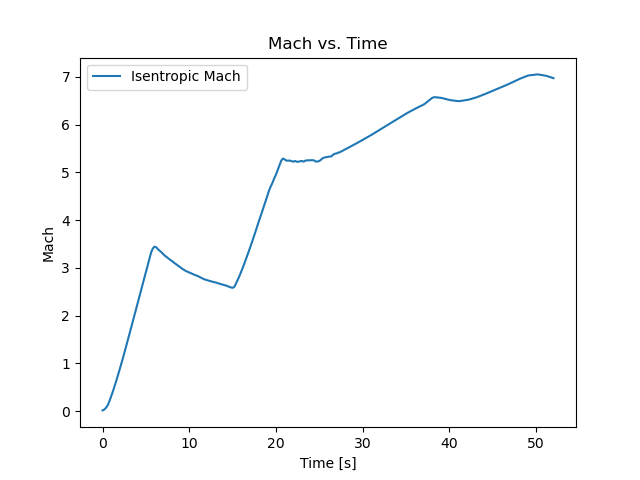
\includegraphics[scale=.7]{../../images/problem_1/Mach_correct_vs_Time.png}
    \caption{Mach vs. Time using accurate air temperature values}
    \label{Mach_correct}
\end{figure}

Figure \ref{Mach_298} shows the freestream Mach versus time, calculated using a constant air temperature of \(T=298\,\unit{\kelvin}\).

\begin{figure}[h]
    \centering
    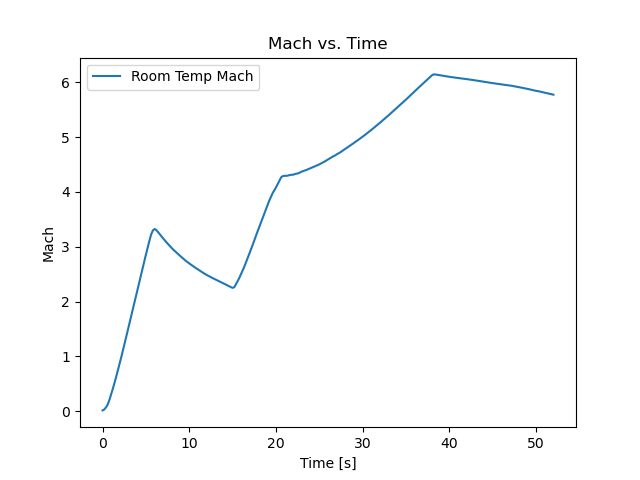
\includegraphics[scale=.7]{../../images/problem_1/Mach_298_vs_Time.png}
    \caption{Mach vs. Time using constant room temperature air}
    \label{Mach_298}
\end{figure}

Figure \ref{Mach} shows both calculated Mach histories including the abosolute error magnitude.

\begin{figure}[h]
    \centering
    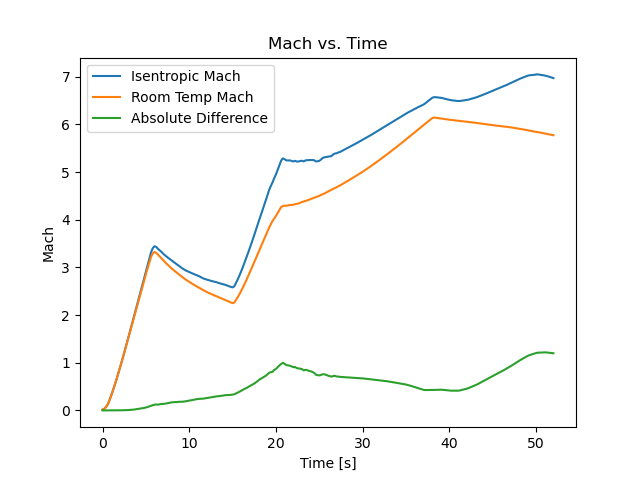
\includegraphics[scale=.7]{../../images/problem_1/Mach_vs_Time.png}
    \caption{Mach vs. Time comparison with absolute error magnitude}
    \label{Mach}
\end{figure}

Figure \ref{Mach_error} shows the absolute \% error between both methods of calculating Mach number.

\begin{figure}[h]
    \centering
    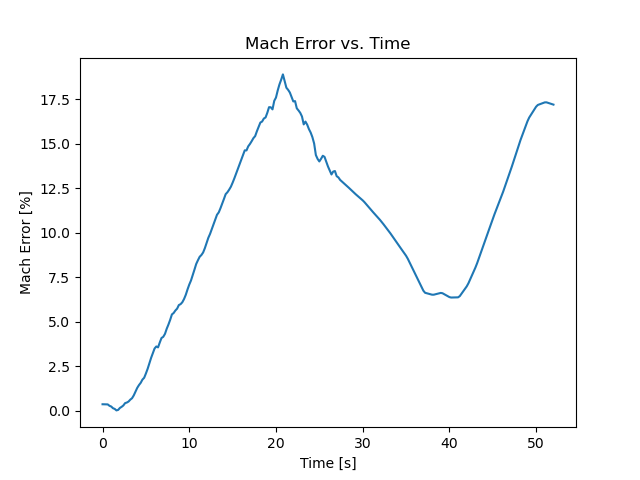
\includegraphics[scale=.7]{../../images/problem_1/Mach_Error_vs_Time.png}
    \caption{Absolute \% Mach error vs. Time}
    \label{Mach_error}
\end{figure}

\discussion{}

Using a constant room temperature value for air throughout all points of the trajectory would induce dramatic amounts of error to any subsequent calculations relevant to the experiments present on the vehicle.
Examining figure \ref{Mach_error}, we see up to 17.5 \% error between the methods of Mach calculation, corresponding to over an entire Mach number of difference at \(t=20\,\unit{\s}\).
There is no reason to use constant room temperature values when atmospheric conditions are so easily obtained and the difference in calculation method is nonexistent. 
To obtain \textbf{any} amount of accuracy, we must use accurate atmospheric conditions.

\clearpage

\problempart{b} 

Prove that use of compressible-flow equations is more appropriate than use of Bernoulli for analyzing the vehicle trajectory.
Provide a plot of \(\rho_\infty/\rho_0\) versus time and identify the first point in time at which flow is considered compressible.
Provide a plot of \(p_0\) versus time caculated both using isentropic relations and Bernoulli's equation.
Are there times where the total pressure values agree?
If so, when and why?
Mathematically prove that for \(M<<1\) the isentropic equation for \(p_0/p_\infty\) becomes exactly the Bernoulli equation.

\givens{}
Flight data from trajectory.

\assumptions{}
Air can be treated as an ideal gas with constant specific heats throughout the entire trajectory (i.e., CPG).
Isentropic flow.
\(\gamma_{air} = 1.4\). 
\(R_{air} = 287 \, \unit{\joule/\kilogram\cdot\kelvin}\). 
The flow around the vehicle can be treated as inviscid.

\solution{}

The isentropic flow relation for total-to-static density is given by:

\[
    \frac{\rho_0}{\rho_\infty} = \left({1 + \frac{\gamma-1}{2} M_\infty^2}\right) ^ {\frac{1}{\gamma-1}}   
\]

Obtaining \(\rho_\infty/\rho_0\) involves a simple reciprocal.

\begin{figure}[h]
    \centering
    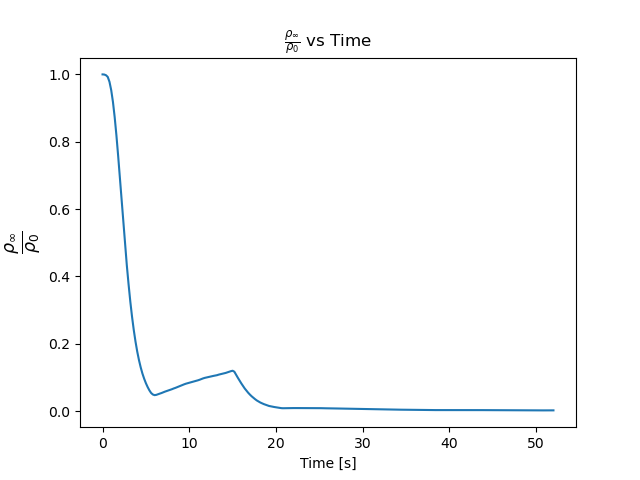
\includegraphics[scale=.7]{../../images/problem_1/rho_rho_t_vs_Time.png}
    \caption{foo}
    \label{rho_rho_t_time}
\end{figure}

\begin{figure}[h]
    \centering
    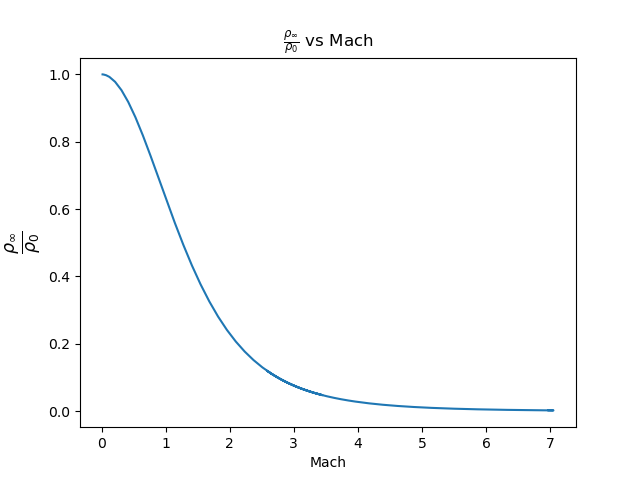
\includegraphics[scale=.7]{../../images/problem_1/rho_rho_t_vs_Mach.png}
    \caption{foo}
    \label{rho_rho_t_vs_Mach}
\end{figure}

\begin{figure}[h]
    \centering
    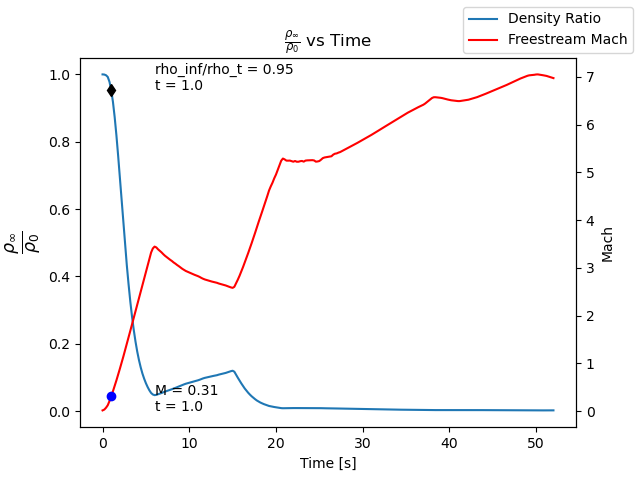
\includegraphics[scale=.7]{../../images/problem_1/rho_rho_t_and_Mach_vs_Time_marked.png}
    \caption{foo}
    \label{rho_rho_t_vs_Mach}
\end{figure}

\begin{figure}[h]
    \centering
    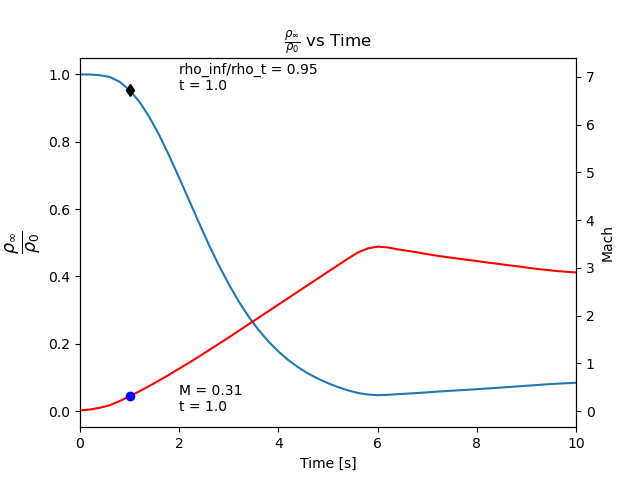
\includegraphics[scale=.7]{../../images/problem_1/rho_rho_t_and_Mach_vs_Time_marked_zoom.png}
    \caption{foo}
    \label{rho_rho_t_vs_Mach}
\end{figure}

\textbf{Blah blah blah calculating total pressure two ways.
They match sometimes. 
Beginning and end.}

\begin{figure}[h]
    \centering
    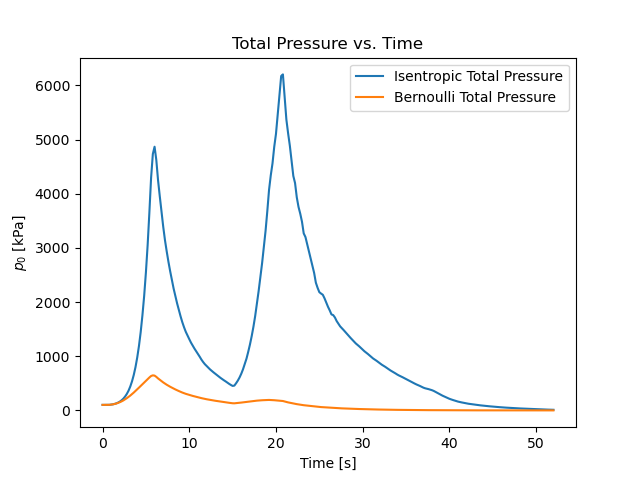
\includegraphics[scale=.7]{../../images/problem_1/Pt_vs_Time_Isen_Bernoulli.png}
    \caption{foo}
    \label{rho_rho_t_vs_Mach}
\end{figure}

\[
    \left({1 + x}\right)^\alpha \approx 1 + \alpha x  
\]

\[
    \frac{p_0}{p_\infty} = {\left({1 + \frac{\gamma-1}{2}M_\infty^2}\right)} ^ {\frac{\gamma}{\gamma-1}}  
\]

\[
    \frac{p_0}{p_\infty} = 1 + \left({\frac{\gamma-1}{2}M_\infty^2}\right) \left({\frac{\gamma}{\gamma-1}}\right)
\]

\[
    \frac{p_0}{p_\infty} = 1 + \left({\frac{\gamma}{2}M_\infty^2}\right) 
\]

\[
    \frac{p_0}{p_\infty} = 1 + \left({\frac{\gamma}{2}}\right)\left({{\frac{u_\infty}{a}}}\right)^2 
\]

\[
    \frac{p_0}{p_\infty} = 1 + \left({\frac{\gamma}{2}}\right)\left({{\frac{u_\infty^2}{\gamma R T_\infty}}}\right) 
\]

\[
    \frac{p_0}{p_\infty} = 1 + \frac{u^2}{2RT_\infty}
\]

\[
    \frac{p_0}{p_\infty} = 1 + \frac{\rho_\infty u^2}{2p_\infty}
\]

\[
    p_0 = p_\infty + \frac{1}{2} \rho_\infty u^2
\]

\end{document}